\chapter{Induction}

\section{Intuition for Uniqueness}

The principles of induction and recursion do more than guarantee the existence of certain functions; they completely characterize them by providing a uniqueness principle. Here we present two examples: natural numbers and lists.

Recall that the type $\N$ of natural numbers has two constructors
\begin{itemize}
    \item $0\colon\N$
    \item $\fun{succ}\colon\N\to\N$.
\end{itemize}
A similar example is the type $\fun L_A$ of finite lists of elements of some type $A$, which has constructors
\begin{itemize}
    \item $\fun{nil}\colon\fun L_A$
    \item $\fun{cons}\colon A\to\fun L_A\to\fun L_A$,
\end{itemize}
where $\fun{nil}$ represents the empty list, and $\fun{cons}(a,\ell)$ the list with head $a$ and tail~$\ell$.

The induction principle for this type states that, given a family $E\colon\fun L_A\to\univ$, to construct a dependent function
\[
    f\colon\prod_{\ell\colon\fun L_A}E(\ell),
\]
it is sufficient to provide the following data:
\begin{itemize}
    \item\phantomsection\label{itm:list-induction} a term $e_{\fun{nil}}\colon E(\fun{nil})$ and
    \item a dependent function $e_{\fun{cons}}\colon\prod_{a\colon A}\prod_{\ell\colon\fun L_A}E(\ell)\to E(\fun{cons}(a,\ell))$.
\end{itemize}
This principle also specifies that the constructed function $f$ computes as expected on the constructors, meaning that we have the definitional equalities
\begin{equation}\label{eq:list-recurrences}
    f(\fun{nil})\equiv e_{\fun{nil}}
    \quad\text{and}\quad
    f(\fun{cons}(a,\ell))
        \equiv e_{\fun{cons}}(a,\ell,f(\ell)).
\end{equation}

\begin{xmpl}\label{xmpl:list-append}
    To define the function
    \[
        \fun{append}\colon\fun L_A\to\fun L_A\to\fun L_A
    \]
    that joins two lists, we define:
    \begin{itemize}
        \item the motive $E(\ell)\defeq\fun L_A\to\fun L_A$,
        \item $e_{\fun{nil}}\defeq\id_{\fun L_A}$, and
        \item $e_{\fun{cons}}(a,\ell,g)\defeq\lambda y.\,\fun{cons}(a,g(y))$.
    \end{itemize}
    Then $\fun{append}\defeq\fun{ind}_{\fun L_A}(E,e_{\fun{nil}},e_{\fun{cons}})$ satisfies
    \[
        \fun{append}(\fun{nil},y)\equiv y
    \]
    and
    \[
        \fun{append}(\fun{cons}(a,\ell),y)
        \equiv
        \fun{cons}(a,\fun{append}(\ell,y)).
    \]
\end{xmpl}

\begin{thm}\label{thm:N-induction-uniqueness}
    Let\/ $f,g\colon\prod_{x\colon\N}E(x)$ be functions satisfying the recurrences
    \[
        e_z\colon E(0)
        \quad\text{and}\quad
        e_s\colon\prod_{n\colon\N}E(n)\to E(\fun{succ}(n))
    \]
    up to propositional equality. That is, assume that
    \[
        f(0)\eq{E(0)}e_z
        \quad\text{and}\quad
        g(0)\eq{E(0)}e_z,
    \]
    and that
    \begin{align*}
        \prod_{n\colon\N}
            f(\fun{succ}(n))
            &\eq{E(\fun{succ}(n))}
            e_s(n,f(n))
    \intertext{and}
        \prod_{n\colon\N}
            g(\fun{succ}(n))
            &\eq{E(\fun{succ}(n))}
            e_s(n,g(n)).
    \end{align*}
    Then\/ $f\sim g$.
\end{thm}

\begin{proof}
    Let $C\colon\N\to\univ$ be the type family defined by $C(n)\defeq f(n)\eq{E(n)}g(n)$. To prove the theorem, it suffices to produce a dependent function in $\prod_{n\colon\N}C(n)$.

    \needspace{2\baselineskip}
    By the induction principle of $\N$, we need to provide the following data:
    \begin{itemize}
        \item a term $c_z\colon C(0)$ and
        \item a function $c_s\colon\prod_{n\colon\N}C(n)\to C(\fun{succ}(n))$.
    \end{itemize}
    The first part of our hypothesis gives us paths 
    \[
        p_0\colon f(0)\eq{E(0)}e_z
        \quad\text{and}\quad
        q_0\colon g(0)\eq{E(0)}e_z,
    \]
    which we can use to produce $c_z\defeq p_0\ct q_0^{-1}\colon C(0)$.

    To define $c_s$, given $n\colon\N$ and $h\colon C(n)$, we must construct $c_s(n,h)\colon C(\fun{succ}(n))$. Since $h\colon f(n)\eq{E(n)}g(n)$, we can use the action on paths to obtain
    \[
        \fun{ap}_{e_s(n,\dummy)}(h)\colon
            e_s(n,f(n))\eq{E(\fun{succ}(n))} e_s(n,g(n)).
    \]
    The second part of the hypothesis yields paths
    \[
        p_n\colon
            f(\fun{succ}(n))
            \eq{E(\fun{succ}(n))}
            e_s(n,f(n))
    \]
    and
    \[
        q_n\colon
            g(\fun{succ}(n))
            \eq{E(\fun{succ}(n))}
            e_s(n,g(n)).
    \]
    Concatenating these paths yields
    \[
        p_n\ct\fun{ap}_{e_s(n,\dummy)}(h)\ct q_n^{-1}\colon
            f(\fun{succ}(n))
            \eq{E(\fun{succ}(n))}
            g(\fun{succ}(n)),
    \]
    which is definitionally equal to $C(\fun{succ}(n))$. To complete the proof, we set $c_s(n,h)$ to be this concatenation.
\end{proof}

\begin{rem}\label{rem:List-induction-uniqueness}
    A similar theorem holds for lists: \textit{If\/ $f,g\colon\prod_{x\colon\fun L_A}E(x)$ propositionally satisfy the recurrences \eqref{eq:list-recurrences}, then\/ $f\sim g$}.

    The proof proceeds exactly as in the theorem, introducing
    \[
        C(\ell)\defeq f(\ell)\eq{E(\ell)}g(\ell),
    \]
    and then defining $c_{\fun{nil}}$ by concatenating the paths
    \[
        f(\fun{nil})\eq{E(\fun{nil})}e_{\fun{nil}}
        \quad\text{and}\quad
        g(\fun{nil})\eq{E(\fun{nil})}e_{\fun{nil}}.
    \]
    The definition of $c_{\fun{cons}}(a,\ell,\eta)$ comes from
    \[
        \fun{ap}_{e_{\fun{cons}}(a,\ell,\dummy)}(\eta)
            \colon e_{\fun{cons}}(a,\ell,f(\ell))
                \eq{E(\fun{cons}(a,\ell))}
                e_{\fun{cons}}(a,\ell,g(\ell))
    \]
    and the equalities
    \[
        f(\fun{cons}(a,\ell))\eq{E(\fun{cons}(a,\ell))}
        e_{\fun{cons}}(a,\ell,f(\ell))
    \]
    and
    \[
        g(\fun{cons}(a,\ell))\eq{E(\fun{cons}(a,\ell))}
        e_{\fun{cons}}(a,\ell,g(\ell)).
    \]
\end{rem}

Suppose we have a different construction of the natural numbers:
\begin{itemize}
    \item $0'\colon\N'$
    \item $\fun{succ'}\colon\N'\to\N'$,
\end{itemize}
along with an induction principle
\[
    \fun{ind}_{\N'}\colon\prod_{E\colon\N'\to\univ}
        E(0')\to\Bigl(\prod_{n'\colon\N'}E(n') \to E(\fun{succ'}(n'))\Bigr)
        \to \prod_{n'\colon\N'}E(n')
\]
and the definitional equalities
\begin{align*}
    \fun{ind}_{\N'}(E, e_0, e_s, 0') &\defeq e_0,\\
    \fun{ind}_{\N'}(E, e_0, e_s, \fun{succ'}(n')) &\defeq e_s(n', \fun{ind}_{\N'}(E, e_0, e_s, n')).
\end{align*}
We can use the constant families $E(n)\defeq\N'$ and $E'(n')\defeq\N$ to define
\begin{align*}
    f\colon\N\to\N'&\defeq\fun{ind}_\N
        (
            E,
            0',
            \lambda n.\,\fun{succ'}
        )
\intertext{and}
    g\colon\N'\to\N&\defeq\fun{ind}_{\N'}
        (
            E',
            0,
            \lambda n'.\,\fun{succ}
        ).
\end{align*}
First, observe that
\[
    g\circ f(0)\equiv g(0')\equiv 0\equiv\id_\N(0)
\]
and also
\[
    g\circ f(\fun{succ}(n))
        \equiv g(\fun{succ'}(f(n)))
        \equiv \fun{succ}(g(f(n)))
        \equiv \fun{succ}(g\circ f(n)).
\]
Since $\id_\N(\fun{succ}(n))\equiv\fun{succ}(\id_\N(n))$, by setting $e_s(x,y)\defeq \fun{succ}(y)$ we can rewrite the equivalences above as
\[
    g\circ f(\fun{succ}(n))\equiv e_s(n,g\circ f(n))
    \quad\text{and}\quad
    \id_\N(\fun{succ}(n))\equiv e_s(n,\id_\N(n)).
\]
Therefore, by Theorem~\ref{thm:N-induction-uniqueness}, we obtain a homotopy $\vartheta\colon g\circ f\sim\id_{\N}$.

A symmetric argument yields a homotopy $\eta\colon f\circ g\sim\id_{\N'}$. Consequently, $f$ and $g$ are quasi-inverses and so $\N\simeq\N'$. Thus, the univalence axiom constructs a path $\N\eq{\univ}\N'$.

\begin{xmpl}\label{xmpl:N-from-List(1)}
    A concrete example of an alternative construction of $\N$ is the following:
    \begin{itemize}
        \item $\N'\defeq\fun{List}(\fun1)$,
        \item $0'\defeq\fun{nil}$, and
        \item $\fun{succ'}(\ell)\defeq\fun{cons}(\fstar,\ell)$,
    \end{itemize}
    with the induction principle
    \begin{align*}
        \fun{ind}_{\N'}&\colon\prod_{E\colon\N'\to\univ}
            E(\fun{nil})
            \to\Bigl(\prod_{\ell\colon\N'}E(\ell)
                \to E(\fun{succ'}(\ell))\Bigr)
            \to \prod_{y\colon\N'}E(y)\\
        \fun{ind}_{\N'}
            (
                E,
                e_{\fun{nil}},
                g
            )
        &\defeq
        \fun{ind}_{\fun{List}(\fun1)}
            (
                E,
                e_{\fun{nil}},
                \lambda z\colon\fun1.\,g_z
            ),
    \end{align*}
    which fulfills the requirements of $\fun{ind}_{\fun{List}(\fun1)}$ because
    \[
        (\lambda z\colon\fun1.\,g_z)\colon
            \prod_{z\colon\fun1}\;\prod_{\ell\colon\fun{List}(\fun1)}E(\ell)\to E(\fun{cons}(z,\ell))
    \]
    is defined as follows. For a given path $p_z\colon\fstar\eq{\fun1}z$, the action on paths yields
    \[
        \fun{ap}_{\fun{cons}(\dummy,\ell)}(p_z)\colon
        \fun{cons}(\fstar,\ell)\eq{\N'}\fun{cons}(z,\ell).
    \]
    Since $g(\ell)\colon E(\ell)\to E(\fun{cons}(\fstar,\ell))$, we can define $g_z(\ell)$ by composing $g(\ell)$ with the transport function along this path:
    \[
        g_z(\ell)\defeq
            \fun{transport}^E(\fun{ap}_{\fun{cons}(\dummy,\ell)}(p_z), \dummy)
                \circ g(\ell).
    \]
\end{xmpl}

\begin{rem}
    The same ideas can be applied to other inductive types. For instance, as shown in Exercise~\ref{exr:A+B-from-rec2}, the coproduct $A+B$ can be implemented as
    \[
        A\oplus B\defeq\sum_{x\colon\fun2}
            \fun{rec}_{\fun2}(\univ,A,B,x)
    \]
    with constructors
    \begin{itemize}
        \item $\fun{in}_A(x)\defeq\dep{0_{\fun2},x}$ and
        \item $\fun{in}_B(y)\defeq\dep{1_{\fun2},y}$,
    \end{itemize}
    which are well-defined because $\fun{rec}_{\fun2}(\univ,A,B,0_{\fun2})\equiv A$ and $\fun{rec}_{\fun2}(\univ,A,B,1_{\fun2})\equiv B$.
    
    In this case, the induction principle for $A\oplus B$ is given by
    \[
        \fun{ind}_{A\oplus B}(C,g_0,g_1)
        \defeq
        \fun{ind}_{\sum_{t\colon\fun2}\fun{rec}_{\fun2}(\univ,A,B,t)}
        \bigl(
            C,
            \fun{ind}_{\fun2}(D,g_0,g_1)
        \bigr),
    \]
    where the motive $D\colon\fun2\to\univ$ is defined as
    \[
        D(t)\defeq\prod_{z\colon\fun{rec}_{\fun2}(\univ,A,B,t)}C(\dep{t,z}).
    \]
    The associated computation rules evaluate as follows:
    \begin{align*}
        \fun{ind}_{A\oplus B}(C,g_0,g_1,\fun{in}_A(x)) &\equiv g_0(x),\\
        \fun{ind}_{A\oplus B}(C,g_0,g_1,\fun{in}_B(y)) &\equiv g_1(y).
    \end{align*}
    Since $A\oplus B$ satisfies the same induction principle as $A+B$, they are canonically equivalent.
\end{rem}

\section{Well-Founded Trees}

\textsl{Well-founded trees}, a.k.a.~\textsl{$\fun W$-trees}, generalize inductive data structures such as natural numbers and lists. The term ``well-founded'' means that there are no infinite downward paths in these trees.

A $\fun W$-tree has two basic ingredients: a \textsl{label} type $A$ and an \textsl{arity} type family $B\colon A\to\univ$. The $\fun W$-type models $\fun W$-trees. It is denoted $\fun W_{x\colon A}B(x)$, or simply $\fun W_AB$.

The term-construction process has two steps. First, we choose a label $a\colon A$ for the root. The type $A$ encodes the possible node constructors.

Second, the type family $B(a)$ dictates the branches hanging from that node. If $B(a)$ is the empty type, the node is a leaf: it has zero branches. If $B(a)$ is the boolean type, the node has two branches, and so forth. 

If the node has branches, a fully formed subtree hangs from each of them. As illustrated below, the branches are indexed by the elements $b_1,b_2,\dots,b$ of $B(a)$. The function $f\colon B(a)\to\fun W_{x\colon A}B(x)$ attaches a subtree $f(b)$ to each branch, represented by the dotted triangles.
\[
    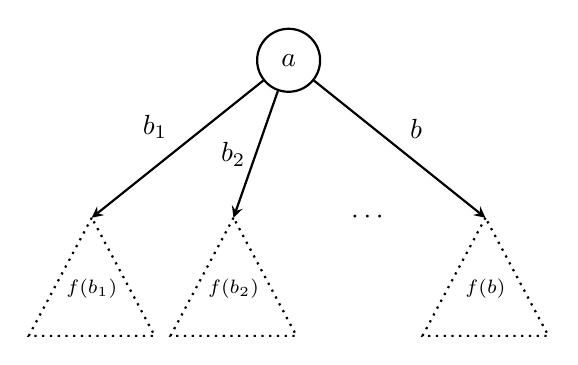
\begin{tikzpicture}[>=stealth, thick]
        % Root node labeled by a in A
        \node[circle, draw, minimum size=8mm] (a) at (0,0) {$a$};
    
        % Apexes of the subtrees
        \coordinate (t1) at (-2.5, -2);
        \coordinate (t2) at (-0.7, -2);
        \coordinate (tb) at (2.5, -2);
    
        % Branches indexed by elements of B(a)
        \draw[->] (a) -- node[above left] {$b_1$} (t1);
        \draw[->] (a) -- node[left] {$b_2$} (t2);
        \draw[->] (a) -- node[above right] {$b$} (tb);
    
        % Ellipsis indicating B(a)-many arguments
        \node at (1, -2) {$\cdots$};
    
        % Dotted triangles representing the well-founded subtrees f(b_i)
        \draw[dotted, thick] (t1) -- ++(-0.8, -1.5) -- ++(1.6, 0) -- cycle;
        \node at (-2.5, -2.9) {$\scriptstyle f(b_1)$};
    
        \draw[dotted, thick] (t2) -- ++(-0.8, -1.5) -- ++(1.6, 0) -- cycle;
        \node at (-0.7, -2.9) {$\scriptstyle f(b_2)$};
    
        \draw[dotted, thick] (tb) -- ++(-0.8, -1.5) -- ++(1.6, 0) -- cycle;
        \node at (2.5, -2.9) {$\scriptstyle f(b)$};
    \end{tikzpicture}
\]
The induction principle of the $\fun W$-type ensures that each of these triangles is itself a well-founded tree. Thus, the branching process repeats inside each triangle and terminates at leaves after a finite number of steps.

Because $\fun W$-types serve as a universal generalization of inductive types, all the distinct constructors of a given type are unified into a single constructor, namely the function:
\begin{equation}\label{eq:sup-constructor}
    \fun{sup}\colon
        \prod_{a\colon A}\;
        \bigl(
            B(a)\to\fun W_AB
        \bigr)
            \to\fun W_AB.
\end{equation}
When a term is built using $\fun{sup}(a,f)$, the label $a\colon A$ acts as the indicator for which constructor is being applied, while the function $f\colon B(a)\to\fun W_AB$ supplies the subtrees required by that specific constructor.

In this way, the single constructor $\fun{sup}$ expresses the behavior of any number of individual constructors by delegating the choice of the operation to the label type~$A$.

\begin{rem}\label{rem:rec(sup)-is-P(W)->W}
    According to \nref{lpar:Sigma-type-rec-and-ind}, the constructor\/ $\fun{sup}$ given by \eqref{eq:sup-constructor} determines a function
    \begin{equation}\label{eq:P(W)->W}
        \fun{rec}_{\sum_{a\colon A}B(a)\to\fun W_AB}
            (
                \fun W_AB,
                \fun{sup}
            )
            \colon
            \Bigl(
                \sum_{a\colon A}B(a)\to\fun W_AB
            \Bigr)
            \to\fun W_AB.
    \end{equation}
\end{rem}

\begin{xmpl}\label{xmpl:W-tree-for-List(X)}
    To illustrate how $\fun W$-trees are appropriate for generalizing inductive types, let us use them to produce a new definition of $\fun L_X$.

    The core idea is that, when using $\fun W$-trees, \textbf{constructors are labeled by elements, and their recursive arguments (if any) by types}. This strictly separates the non-recursive data of a constructor from its recursive structure. The elements act as labels belonging to a type $A$, and the shape of the recursive arguments is dictated by an \textsl{arity} type family $B\colon A\to\univ$.

    In our case, the constructors are $\fun{nil}$ and $\fun{cons}$. Since $\fun{nil}$ carries no non-recursive data, we can associate it to the nullary label $\fstar\colon\fun1$. For $\fun{cons}$, we have two arguments: $x\colon X$ and $\ell\colon\fun L_X$. The first one is not recursive, so we must tag it directly as a label; thus, we use a whole family of unary labels provided by the type $X$ to represent the constructor family $x\mapsto\fun{cons}(x,\dummy)$.

    The second argument $\ell\colon\fun L_X$ is recursive. Since each constructor $\fun{cons}(x,\dummy)$ expects one recursive argument, it is assigned an arity of the unit type $\fun1$. Similarly, since $\fun{nil}$ expects zero recursive arguments, its arity is the empty type~$\fun0$.

    Summarizing, our proposal is to define $A\defeq\fun1+X$ and specify the arity family $B\colon A\to\univ$ by cases: $B(\fun{inl}(\fstar))\defeq\fun0$ and $B(\fun{inr}(x))\defeq\fun1$. In other words, $B(a)\defeq\fun{rec}_{\fun1+X}(\univ,\lambda{\star}.\,\fun0,\lambda{\star}.\,\fun1,a)$.
    \[
        % Generic structure of a cons(x, \ell) node
        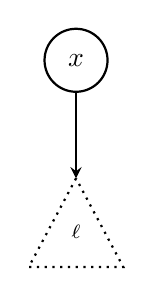
\begin{tikzpicture}[
            scale=0.75,
            >=stealth,
            thick,
            baseline=0]
            % Root node labeled by x in X
            \node[circle, draw, minimum size=8mm] (x) at (0,0) {$x$};
        
            % Apex of the subtree \ell
            \coordinate (t) at (0, -2);
        
            % Single branch indexed by the element of B(x) = 1
            \draw[->] (x) -- node[right] {$\fstar$} (t);
        
            % Dotted triangle representing the well-founded subtree \ell
            \draw[dotted, thick] (t) -- ++(-0.8, -1.5) -- ++(1.6, 0) -- cycle;
            \node at (0, -2.9) {$\scriptstyle \ell$};
        \end{tikzpicture}
        \hspace{3cm}
        % Fully expanded 3-element list
        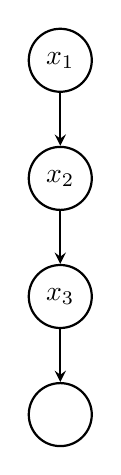
\begin{tikzpicture}[
            scale=0.75,
            >=stealth,
            thick,
            baseline=0]
            % Nodes for the elements of the list (arity 1)
            \node[circle, draw, minimum size=8mm] (x1) at (0,0) {$x_1$};
            \node[circle, draw, minimum size=8mm] (x2) at (0,-2) {$x_2$};
            \node[circle, draw, minimum size=8mm] (x3) at (0,-4) {$x_3$};
            
            % Leaf node representing nil (arity 0)
            \node[circle, draw, minimum size=8mm] (nil) at (0,-6) {$\fstar$};
        
            % Branches indexed by the single element of the unit type
            \draw[->] (x1) -- node[right] {$\fstar$} (x2);
            \draw[->] (x2) -- node[right] {$\fstar$} (x3);
            \draw[->] (x3) -- node[right] {$\fstar$} (nil);
        \end{tikzpicture}
    \]
    The first graph depicts the recursive step for the constructor\/ $\fun{cons}(x,\ell)$. The root is labeled by\/ $x$, representing\/ $\fun{inr}(x)\colon A$. Since the arity of this label is\/ $B(\fun{inr}(x))\defeq\fun1$, there is exactly one downward edge emerging from the node. This edge is indexed by\/ $\fstar$, and the subtree-assigning function\/ $f\colon\fun1\to\fun W_AB$ attaches the recursive argument by defining\/ $f(\fstar)\defeq\ell$.

    \needspace{2\baselineskip}
    With this, we can formally redefine:
    \begin{itemize}
        \item\phantomsection\label{itm:list-from-W}
        $\fun\fun L'_X\defeq\fun W_{\fun1+X}\fun{rec}_{\fun1+X}(\univ,\lambda{\star}.\,\fun0,\lambda{\star}.\,\fun1)$,
        \item $\fun{nil'}\defeq\fun{sup}(\fun{inl}(\fstar),\fun{rec}_{\fun0}(\fun\fun L'_X))$, and
        \item $\fun{cons'}(x,\ell')\defeq\fun{sup}(\fun{inr}(x),\lambda{\fstar}.\,\ell')$.
    \end{itemize}

    The second graph illustrates a list of three elements. Each node $x_i$ has arity $\fun1$, creating a single downward branch. The list terminates at the node representing the $\fun{nil}$ constructor. This leaf node is labeled by $\fstar$, which stands for $\fun{inl}(\fstar)\colon A$. Because its arity is the empty type, no edges depart from it.
\end{xmpl}

\begin{xmpl}\label{xmpl:W-tree-for-N}
    To formalize the natural numbers using $\fun W$-trees, we must define the label type $A$ to represent two constructors: $0$ and $\fun{succ}$.
    
    Since the former has no recursive arguments, we can consider $\fun1$ for labeling it. The latter has a single argument $n$, which is recursive. So, $\fun1$ would also work for labeling the $\fun{succ}$ constructor. Thus, $\fun1+\fun1$ is appropriate for $A$, and this can be abbreviated by setting $A\defeq\fun2$.
    
    The arity family $B\colon A\to\univ$ needs to represent the recursive arguments of each constructor. Thus, we define it by
    \begin{align*}
        B(0_{\fun2})&\defeq\fun0,\\
        B(1_{\fun2})&\defeq\fun1.
    \end{align*}
    Thus, the arity function can be specified as
    \[
        B\defeq\fun{rec}_{\fun2}(\univ,\fun0,\fun1).
    \]
    The subtree-assigning function $f\colon B(a)\to\fun W_{\fun2}B$ depends on the constructor being encoded.
    
    For the base case $0$, we have $f_0\defeq\fun{rec}_{\fun0}(\fun W_{\fun2}B)$.
    
    For the inductive step $\fun{succ}(n)$, we have $f_{\fun{succ}}\defeq\lambda{\fstar}.\,n$.

    In summary:
    \begin{itemize}
        \item $\N'\defeq\fun W_{\fun2}B$,
        \item $0'\defeq\fun{sup}(0_{\fun2},\fun{rec}_{\fun0}(\N'))$, and
        \item $\fun{succ}'(n)\defeq\fun{sup}(1_{\fun2},\lambda{\fstar}.\,n)$.
    \end{itemize}
    Here is a graph showing the recursive constructor $\fun{succ}$ on the left. On the right, we have a representation of $2\defeq\fun{succ}(\fun{succ}(0))$:
    \[
        % Recursive step for succ(n)
        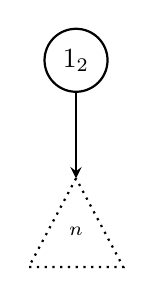
\begin{tikzpicture}[
            scale=0.75,
            >=stealth,
            thick,
            baseline=0]
            % Root node labeled by x in X
            \node[circle, draw, minimum size=8mm] (x) at (0,0) {$1_{\fun2}$};
        
            % Apex of the subtree \ell
            \coordinate (t) at (0, -2);
        
            % Single branch indexed by the element of B(x) = 1
            \draw[->] (x) -- node[right] {$\fstar$} (t);
        
            % Dotted triangle representing the well-founded subtree \ell
            \draw[dotted, thick] (t) -- ++(-0.8, -1.5) -- ++(1.6, 0) -- cycle;
            \node at (0, -2.9) {$\scriptstyle n$};
        \end{tikzpicture}
        \hspace{3cm}
        % Concrete tree for the number 2
        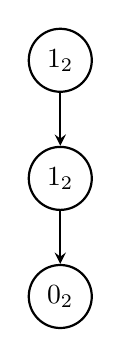
\begin{tikzpicture}[
            level distance=2.0cm,
            wnode/.style={circle, draw, minimum size=8mm},
            edge from parent/.style={draw, ->},
            scale=0.75,
            >=stealth,
            thick,
            baseline=0]
            \node[wnode] {$1_{\fun2}$}
                child {
                    node[wnode] {$1_{\fun2}$}
                    child {
                        node[wnode] {$0_{\fun2}$}
                        edge from parent node[right] {$\fstar$}
                    }
                    edge from parent node[right] {$\fstar$}
                };
        \end{tikzpicture}
    \]
\end{xmpl}

\section{{\normalfont\textsf W}-Types}

\begin{defn}
    The formal definition of the $\fun W$-type is given by its rules for formation, introduction, elimination, and computation. Let $A\colon\univ$ be a type and $B\colon A\to\univ$ be a type family.
    
    \textsc{Formation:} The type is formed by the binder $\fun W$, yielding a type in the universe:
    \[
        \fun W_{x\colon A}B(x)\colon\univ.
    \]
    
    \textsc{Introduction:} The elements of the $\fun W$-type are built using the constructor $\fun{sup}$. Given a label $a\colon A$ and a subtree-assigning function $f\colon B(a)\to \fun W_AB$, we can form a new tree $\fun{sup}(a,f)$, where
    \begin{equation}\label{eq:W-constructor}
        \fun{sup}\colon
            \prod_{a\colon A}\;
            \bigl(
                B(a)\to\fun W_AB
            \bigr)
                \to\fun W_AB.
    \end{equation}
    
    \textsc{Elimination:} To construct a dependent function over the\/ $\fun W$-type, we use its induction principle. Given a motive\/ $E\colon\fun W_AB\to\univ$, we must provide an inductive step function\/ $e_s$ that constructs a term in\/ $E(\fun{sup}(a,\phi))$ assuming we already have terms in\/ $E(\phi(b))$ for all\/ $b\colon B(a)$. The required signature for\/ $e_s$ is
    \begin{equation}\label{eq:ind_W-step-function}
        e_s\colon\prod_{a\colon A}\;\prod_{\phi\colon B(a)\to \fun W_AB}
            \Bigl(\prod_{b\colon B(a)}E(\phi(b))\Bigr)
            \to E(\fun{sup}(a,\phi)).
    \end{equation}
    With this data, the induction principle produces a dependent function
    \begin{equation}\label{eq:W-induction-function}
        \fun{ind}_{\fun W}(E, e_s)
            \colon\prod_{w\colon \fun W_AB}E(w).
    \end{equation}
    As a special case, when the motive is a constant type family\/ $E(w)\defeq C$ for some carrier type\/ $C\colon\univ$, the inductive step function simplifies to a curried structure map\/ $s_C\colon\prod_{a\colon A}(B(a)\to C)\to C$. The induction principle then reduces to the non-dependent \textsl{recursor}
    \begin{equation}\label{eq:rec_W}
        \fun{rec}_{\fun W}(C, s_C)
            \colon \fun W_AB\to C.
    \end{equation}
    To see how the inductive step function simplifies when the motive is a constant type family $E(w)\defeq C$, we can trace the definitional equalities and equivalences of its signature. Fixing $a\colon A$, we have
    \begin{align*}
            \prod_{\phi\colon B(a)\to\fun W_AB}\,
            \Bigl(\prod_{b\colon B(a)}E(\phi(b))\Bigr)
            \to E(\fun{sup}(a,\phi)
        &\equiv
            \prod_{\phi\colon B(a)\to \fun W_AB}\,
            \Bigl(\prod_{b\colon B(a)}C\Bigr)
            \to C\\
        &\equiv
            \prod_{\phi\colon B(a)\to\fun W_AB}
            \!\!\!(B(a)\to C)\to C.
    \end{align*}
    The final expression provides access to both the recursive results $B(a)\to C$ and the original subtrees $\phi\colon B(a)\to\fun W_AB$. However, since $(B(a)\to C)\to C$ does not depend on the original trees in $\fun W_AB$, we can drop the unused parameter $\phi\colon B(a)\to\fun W_AB$ to obtain the curried structure map:
    \[
        s_C\colon\prod_{a\colon A}(B(a)\to C)\to C.
    \]

    \textsc{Computation:} The eliminators compute by evaluating the step function on the components of the\/ $\fun{sup}$ constructor. For the induction principle, the computation rule is the definitional equality
    \begin{equation}\label{eq:ind_W-computation-rule}
        \fun{ind}_{\fun W}(E,e_s)(\fun{sup}(a,\phi)) 
            \equiv
            e_s(a,\phi,\fun{ind}_{\fun W}(E,e_s)\circ\phi).
    \end{equation}
    Accordingly, the computation rule for the recursor is
    \begin{equation}\label{eq:rec_W-computation-rule}
        \fun{rec}_{\fun W}(C,s_C)(\fun{sup}(a,\phi))
            \equiv s_C(a,\fun{rec}_{\fun W}
                (
                    C,s_C
                )\circ\phi).
    \end{equation}
\end{defn}

\begin{xmpl}\label{xmpl:List(X)-induction-from-W-induction}
    To see how this general framework operates in a concrete inductive type, let us continue with Example~\ref{xmpl:W-tree-for-List(X)}. The goal is to derive the induction principle for $\fun L_X$ from the induction principle for $\fun W$-types.

    We must construct the data required by $\fun W$-induction to yield standard list induction. This involves case analysis over the label $a\colon\fun1+X$.

    Suppose $a\equiv\fun{inl}(\fstar)$. In this case, we have $B(a)\equiv\fun0$. Consequently, the associated subtree function is the unique definitional equality $f\equiv\fun{rec}_{\fun0}(\fun W_AB)$. Moreover, $\fun{sup}(a,f)$ is definitionally equal to $\fun{nil}$.

    The inductive hypothesis is a dependent function $g\colon\prod_{b\colon\fun0}E(f(b))$. Because the product runs over the empty type, this type is equivalent to $\fun1$ and contains a unique, trivial inhabitant.

    For this case, the inductive step function of $\fun{ind}_{\fun W}$ needs to map this trivial inhabitant to a term in $E(\fun{sup}(a,f))\equiv E(\fun{nil})$. This is precisely the data required by \hyperref[itm:list-induction]{standard list induction$\,\scriptstyle[\uparrow]$}: a term $e_{\fun{nil}}\colon E(\fun{nil})$.

    In the case where $a\equiv\fun{inr}(x)$, we have $B(a)\equiv\fun1$. Thus, the subtree-assigning function has the signature $f\colon\fun1\to\fun W_{x\colon A}B(x)$. \hyperref[itm:list-from-W]{As established before$\,\scriptstyle[\uparrow]$}, the constructor application $\fun{sup}(a,f)$ is definitionally equal to $\fun{cons}(x,f(\fstar))$.

    The inductive hypothesis is a dependent function $g\colon\prod_{b\colon\fun1}E(f(b))$, which provides a single meaningful term: $g(\fstar)\colon E(f(\fstar))$.

    To complete the definition of $e_s$, we must construct a term in $E(\fun{sup}(a,f))$, which evaluates to $E(\fun{cons}(x,f(\fstar)))$. But this is exactly the data provided by the \hyperref[itm:list-induction]{standard list induction$\,\scriptstyle[\uparrow]$}: a dependent function $e_{\fun{cons}}$ that takes the head $x$, the tail $f(\fstar)$, and the inductive hypothesis $g(\fstar)$, and returns a term in $E(\fun{cons}(x,f(\fstar)))$.

    Consequently, we can fully define the inductive step function $e_s$ by pattern matching on the label $a\colon\fun1+X$:
    \begin{align*}
        e_s(\fun{inl}(\fstar), f, g) &\defeq e_{\fun{nil}}, \\
        e_s(\fun{inr}(x), f, g) &\defeq e_{\fun{cons}}(x, f(\fstar), g(\fstar)).
    \end{align*}
    It follows that the induction principle for lists is simply a specific instance of the induction principle for $\fun W$-types:
    \[
        \fun{ind}_{\fun{List}}(E, e_{\fun{nil}}, e_{\fun{cons}})
            \defeq \fun{ind}_{\fun W}(E, e_s).
    \]
\end{xmpl}

\begin{thm}\label{thm:W-type-induction-uniqueness}
    Let\/ $g,h\colon\prod_{w\colon\fun W_AB}E(w)$ be two functions which satisfy the recurrence
    \[
        e\colon\prod_{a,f}\;
        \Bigl(
            \prod_{b\colon B(a)}E(f(b))
        \Bigr)
        \to E(\fun{sup}(a,f))
    \]
    propositionally, i.e., such that
    \begin{align*}
        \prod_{a,f} g(\fun{sup}(a,f))
            &\eq{E(\fun{sup}(a,f))}
                e(a,f,\lambda b.\,g(f(b))),\\
        \prod_{a,f} h(\fun{sup}(a,f))
            &\eq{E(\fun{sup}(a,f))}
                e(a,f,\lambda b.\,h(f(b))).
    \end{align*}
    Then\/ $g\sim h$.
\end{thm}

\begin{proof}
    Let $C\colon\fun W_AB\to\univ$ be the type family defined by
    \[
        C(w)\defeq g(w)\eq{E(w)}h(w).
    \]
    We must construct a witness for $\prod_{w\colon\fun W_AB}C(w)$. By the induction principle of $\fun W$-types, this reduces to defining a step function \eqref{eq:ind_W-step-function}
    \[
        c_s(a,f)\colon
            (g\circ f\sim h\circ f)
            \to
                \bigl(
                    g(\fun{sup}(a,f))
                    \eq{E(\fun{sup}(a,f))}
                    h(\fun{sup}(a,f))
                \bigr)
    \]
    for $a\colon A$ and $f\colon B(a)\to\fun W_AB$.

    Let $\theta\colon g\circ f\sim h\circ f$. Applying the action on paths of the function
    \[
        e(a,f)\colon
            \Bigl(
                \prod_{b\colon B(a)}E(f(b))
            \Bigr)
            \to E(\fun{sup}(a,f))
    \]
    to the path
    \[
        \fun{funext}(\theta)\colon
            g\circ f
            \eq{\prod_{b\colon B(a)}E(f(b))}
            h\circ f
    \]
    yields
    \[
        \fun{ap}_{e(a,f)}(\fun{funext}(\theta))
            \colon e(a,f,g\circ f)
            \eq{E(\fun{sup}(a,f))}
            e(a,f,h\circ f).
    \]
    By hypothesis, we also have paths
    \begin{align*}
        u(a,f)&\colon g(\fun{sup}(a,f))
        \eq{E(\fun{sup}(a,f))}
        e(a,f,g\circ f)
    \intertext{and}
        v(a,f)&\colon h(\fun{sup}(a,f))
        \eq{E(\fun{sup}(a,f))}
        e(a,f,h\circ f).
    \end{align*}
    Therefore, we can define the target path by concatenation:
    \[
        c_s(a,f,\theta)\defeq u(a,f)
            \ct\fun{ap}_{e(a,f)}(\fun{funext}(\theta))
            \ct v(a,f)^{-1}.
    \]
\end{proof}

\section{Initial Algebras}

\begin{defns}\ 
    \begin{enumerate}[-]
            \item An \textsl{$\fun L_X$-algebra} is a type $C$ provided with an element $c_{\fun{nil}}\colon C$ and a function $c_{\fun{cons}}\colon X\to C\to C$. The type of such algebras is
            \[
                \fun L_X\fun{Alg}\defeq\sum_{C\colon\univ}C\times(X\to C\to C).
            \]
            \item Let $\mathcal C\defeq\dep{C,(c_{\fun{nil}},c_{\fun{cons}})}$ and $\mathcal D\defeq\dep{D, (d_{\fun{nil}}, d_{\fun{cons}})}$ be two $\fun L_X$-algebras. An \textsl{$L_X$-morphism} between them is a map $h\colon C\to D$ such that $h(c_{\fun{nil}})\eq Dd_{\fun{nil}}$ and $h(c_{\fun{cons}}(x,c))\eq Dd_{\fun{cons}}(x,h(c))$ for all $x\colon X$ and $c\colon C$. The type of such morphisms is
        \[
            \fun L_X\Hom(\mathcal C,\mathcal D)\defeq
            \sum_{h}
                \bigl(
                    h(c_{\fun{nil}})
                    \eq D
                    d_{\fun{nil}}
                \bigr)
                \times
                \prod_{x,c}
                    h(c_{\fun{cons}}(x,c))
                    \eq D
                    d_{\fun{cons}}(x, h(c)).
        \]
    
        \item An $\fun L_X$-algebra $\mathcal I$ is \textsl{homotopy-initial} (a.k.a.~\textsl{h-initial}) if for any $\fun L_X$ algebra $\mathcal C$ the type of $\fun L_X$-morphisms from $\mathcal I$ to $\mathcal C$ is contractible, i.e.,
        \[
            \fun{isHinit}_{\fun L_X}(\mathcal I)
                \defeq
                \prod_{\mathcal C\colon\fun L_X\fun{Alg}}
                    \fun{isContr}(
                        \fun L_X\Hom(\mathcal I,\mathcal C)
                    )
        \]
        is inhabited.
    \end{enumerate}
\end{defns}

\begin{lem}\label{lem:L_X-morphisms-are-morphisms}
    Given\/ $\fun L_X$-algebras $\mathcal{A}\defeq\dep{A,(a_{\fun{nil}}, a_{\fun{cons}})}$, $\mathcal{B}\defeq\dep{B,(b_{\fun{nil}},b_{\fun{cons}})}$, and\/ $\mathcal{C}\defeq\dep{C,(c_{\fun{nil}}, c_{\fun{cons}})}$, the following hold:
    \begin{enumerate}[a),font=\upshape]
        \item The identity function\/ $\id_A\colon A\to A$ is an\/ $\fun L_X$-morphism from\/ $\mathcal{A}$ to\/ $\mathcal{A}$.
        \item If\/ $f\colon A\to B$ and\/ $g\colon B\to C$ are\/ $\fun L_X$-morphisms, then the composition\/ $g\circ f\colon A\to C$ is an\/ $\fun L_X$-morphism from\/ $\mathcal{A}$ to\/ $\mathcal{C}$.
        \item If\/ $f\colon A\to B$ is an\/ $\fun L_X$-morphism and\/ $g\colon B\to A$ is a quasi-inverse of\/ $f$, then the quasi-inverse\/ $g$ is an\/ $\fun L_X$-morphism from\/ $\mathcal{B}$ to\/ $\mathcal{A}$.
    \end{enumerate}
\end{lem}

\begin{proof}\ 
    \begin{enumerate}[a)]
        \item We need to show that $\id_A(a_{\fun{nil}})=a_{\fun{nil}}$ and $\id_A(a_{\fun{cons}}(x, a))=a_{\fun{cons}}(x, \id_A(a))$ for all $x\colon X$ and $a\colon A$. Both equalities hold definitionally.
        
        \item For the base case, we have
        \[
            (g\circ f)(a_{\fun{nil}})
                \equiv g(f(a_{\fun{nil}}))
                \eq Cg(b_{\fun{nil}})
                \eq Cc_{\fun{nil}}.
        \]
        For the inductive step, let $x\colon X$ and $a\colon A$. Then,
        \begin{align*}
            (g\circ f)(a_{\fun{cons}}(x,a))
                &\equiv g(f(a_{\fun{cons}}(x,a)))\\
                &\eq Cg(b_{\fun{cons}}(x,f(a)))\\
                &\eq Cc_{\fun{cons}}(x,g(f(a)))\\
                &\equiv c_{\fun{cons}}(x,(g\circ f)(a)).
        \end{align*}
        
        \item We have homotopies $\eta\colon f\circ g\sim\id_B$ and $\vartheta\colon g\circ f\sim\id_A$. We must show that $g$ preserves the algebra constructors. For the base case, we apply $\fun{ap}_g$ to the equality $f(a_{\fun{nil}})\eq Bb_{\fun{nil}}$ to obtain $g(f(a_{\fun{nil}}))\eq Ag(b_{\fun{nil}})$. By the homotopy $\vartheta$, we know $g(f(a_{\fun{nil}}))\eq Aa_{\fun{nil}}$. Transitivity of equality thus yields $g(b_{\fun{nil}})\eq Aa_{\fun{nil}}$.
        
        For the inductive step, let $x\colon X$ and $b\colon B$. Since $f$ is a $\fun L_X$-morphism we have $f(a_{\fun{cons}}(x,g(b)))\eq Bb_{\fun{cons}}(x, f(g(b)))$. The homotopy $\eta$ implies $f(g(b))\eq Bb$. Then substitution gives
        \[
            f(a_{\fun{cons}}(x,g(b)))
            \eq Bb_{\fun{cons}}(x,b).
        \]
        Applying $g$ to both sides yields
        \[
            g(f(a_{\fun{cons}}(x,g(b))))
            \eq Ag(b_{\fun{cons}}(x,b)).
        \]
        By the homotopy $\vartheta$, the \lhs is equal to $a_{\fun{cons}}(x,g(b))$. Therefore, we conclude
        \[
            a_{\fun{cons}}(x,g(b))
            \eq Ag(b_{\fun{cons}}(x,b)),
        \]
        which shows that $g$ is an $\fun L_X$-morphism.\qedhere
    \end{enumerate}
\end{proof}

\begin{thm}
    The type of\/ $h$-initial\/ $\fun L_X$-algebras is a mere proposition.
\end{thm}

\begin{proof}
    Let $\mathcal I$ and $\mathcal J$ be two $h$-initial $\fun L_X$-algebras. Then, $\fun L_X\Hom(\mathcal I,\mathcal J)$ is contractible, hence inhabited by, say, $f\colon\mathcal I\to\mathcal J$. By symmetry, there is also $g\colon\mathcal J\to\mathcal I$. Since  Lemma~\ref{lem:L_X-morphisms-are-morphisms} implies that $g\circ f$ and $\id_{\mathcal I}$ inhabit $\fun L_X\Hom(\mathcal I,\mathcal I)$, which is contractible, $g\circ f\eq{\fun L_X\Hom(\mathcal I,\mathcal I)}\id_{\mathcal I}$. The same reasoning proves that $f\circ g\eq{\fun L_X\Hom(\mathcal J,\mathcal J)}\id_{\mathcal J}$.

    It follows that $f$ and $g$ are quasi-inverses and so $\mathcal I\simeq\mathcal J$. The conclusion follows by the univalence axiom.
\end{proof}

\begin{thm}
    The\/ $\fun L_X$-algebra\/ $\dep{\fun L_X,(\fun{nil},\fun{cons})}$ is homotopy initial.
\end{thm}

\begin{proof}
    Let $\mathcal C\defeq\dep{C,(c_{\fun{nil}},c_{\fun{cons}})}$ be an $\fun L_X$-algebra.

    Define $u\colon\fun L_X\to C$ inductively by
    \begin{itemize}
        \item $u(\fun{nil})\defeq c_{\fun{nil}}$,
        \item $u(\fun{cons}(a,\ell))\defeq c_{\fun{cons}}(a,u(\ell))$.
    \end{itemize}
    By definition, $u$ is an $\fun L_X$-morphism.

    Given any other $\fun L_X$-morphism $v\colon\fun L_X\to C$, we have
    \begin{itemize}
        \item $v(\fun{nil})\eq{C} c_{\fun{nil}}$,
        \item $v(\fun{cons}(a,\ell))\eq{C} c_{\fun{cons}}(a,v(\ell))$.
    \end{itemize}
    Therefore, by Remark~\ref{rem:List-induction-uniqueness}, we deduce that $u\sim v$, hence $u\eq{\fun L_X\Hom(\fun L_X,C)}v$. Consequently, $\fun L_X\Hom(\fun L_X,C)$ is contractible with center $u$.
    %
    
\end{proof}

\begin{cor}
    The\/ $\fun L_{\fun1}$-algebra\/ $\dep{\N, (0, \fun{succ})}$ is homotopy initial.
\end{cor}

\begin{proof}
    By the theorem, the $\fun L_{\fun1}$-algebra $\dep{\fun L_{\fun1}, (\fun{nil}, \fun{cons})}$ is $h$-initial. Since we have established in Example~\ref{xmpl:N-from-List(1)} the equality $\N\eq{\univ}\fun L_{\fun1}$, which identifies $0$ with $\fun{nil}$ and $\fun{succ}(n)$ with $\fun{cons}(\fstar,n)$, this yields a path
    \[
        q\colon
        \dep{\N,(0,\fun{succ})}
        \eq{\fun L_{\fun1}\fun{Alg}}
        \dep{\fun L_{\fun1},(\fun{nil},\fun{cons})}.
    \]
    If we define the type family $Q\colon\fun L_{\fun1}\fun{Alg}\to\univ$ by $Q(\mathcal{A})\defeq\fun{isHinit}_{\fun L_{\fun1}}(\mathcal{A})$, then
    \[
        \fun{transport}^Q(q^{-1}) \colon 
        \fun{isHinit}_{\fun L_{\fun1}}(\dep{\fun L_{\fun1},(\fun{nil},\fun{cons})}) 
        \to 
        \fun{isHinit}_{\fun L_{\fun1}}(\dep{\N,(0,\fun{succ})}).
    \]
    Applying this function to the fact that $\dep{\fun L_{\fun1},(\fun{nil},\fun{cons})}$ is $h$-initial provides the desired inhabitant.
\end{proof}

\begin{defn}
    Let $A\colon\univ$ be a type of labels and $B\colon A\to\univ$ an arity family. A \textsl{polynomial functor} (in normal form) is the type family
    \[
        P(X)\defeq\sum_{a\colon A}(B(a)\to X)
    \]
    for any $X\colon\univ$.
\end{defn}

\begin{rem}
    The notion of polynomial functor can be seen as a generalization of \eqref{eq:P(W)->W}. The polynomial aspect of $P(X)$ becomes clear when $B(a)\to X$ is written as $X^{B(a)}$.
\end{rem}

\begin{defn} 
    The type of \textsl{ $\fun W$-algebras} is
    \[
        \fun W\fun{Alg}(A,B)
            \defeq\sum_{C\colon\univ}\;
                \prod_{a\colon A}(B(a)\to C)\to C.
    \]
    Its terms are dependent pairs $\dep{C,s_C}$, where $s_C\colon\prod_{a\colon A}(B(a)\to C)\to C$ is the \textsl{structure map} of the $\fun W$-algebra.
\end{defn}

\begin{rem}
    A $\fun W$-algebra $\dep{C,s_C}$ admits an \textsl{uncurried variant} $\dep{C,\bar{s}_C}$, where
    \[
        \bar{s}_C\defeq\fun{rec}_{P(C)}(C,s_C)
            \colon P(C)\to C.
    \]
    We will refer to this form as a \textsl{$P$-algebra}.
    
    These two views are interchangeable since $s_C$ can be recovered from $\bar{s}_C$ by the computation rule of the $\Sigma$-type.
\end{rem}

\needspace{2\baselineskip}
\begin{defns}\ 
    \begin{enumerate}[-]
        \item Given $P$-algebras $\dep{C,\bar{s}_C}$ and $\dep{D,\bar{s}_D}$, any map $f\colon C\to D$ induces a function $Pf\colon P(C)\to P(D)$ defined by
        \[
            Pf(\dep{a,\phi})\defeq\dep{a,f\circ\phi},
        \]
        for $a\colon A$ and $\phi\colon B(a)\to C$.
        
        \item A \textsl{ $P$-morphism} from a $P$-algebra $\dep{C,\bar{s}_C}$ to another $\dep{D,\bar{s}_D}$ is a dependent pair $\dep{f,\eta_f}$, where $f\colon C\to D$ and $\eta_f\colon f\circ\bar{s}_C\sim\bar{s}_D\circ Pf$. This homotopy can be visualized in the square:
        \[
            \begin{tikzcd}[font=\small]
                P(C)\arrow[r,"Pf"]
                        \arrow[d,"\bar{s}_C"']
                        \arrow[dr,
                            phantom,
                            "\scriptstyle\eta_f"]
                    &P(D)
                        \arrow[d,"\bar{s}_D"]\\
                C
                        \arrow[r,"f"']
                    &D
            \end{tikzcd}
        \]
        Thus, the type of $P$-morphisms is
        \[
            \fun P\Hom(\dep{C,\bar{s}_C},\dep{D,\bar{s}_D})
                \defeq\sum_{f\colon C\to D}
                    f\circ\bar{s}_C\sim\bar{s}_D\circ Pf.
        \]
        Equivalently, using the curried variants $s_C$ and $s_D$, the homotopy condition is given by a family of identities, making the type of morphisms definitionally equivalent to
        \begin{equation}\label{eq:structure-coherence}
            \sum_{f\colon C\to D}\;
                \prod_{a\colon A}\;
                \prod_{\phi\colon B(a)\to C}
                    f(s_C(a,\phi))\eq Ds_D(a,f\circ\phi).
        \end{equation}
        We will denote the type of $\fun W$-morphisms by $\fun W\Hom(\dep{C,s_C},\dep{D,s_D})$, or $\fun W\Hom(C,D)$ for short, if the context permits.

        \item A $\fun W$-algebra $\dep{I,s_I}$ is \textsl{$h$-initial} if the type
        \[
            \fun{isHinit}_{\fun W}(A,B,\dep{I,s_I})
            \defeq
            \prod_{\dep{C,s_C}\colon\fun W\fun{Alg}(A,B)}
            \!\!\!\fun{isContr}
            \bigl(
                \fun W\Hom(I,C)
            \bigr)
        \]
        is inhabited.
    \end{enumerate}
\end{defns}

\begin{defn}
    For a $\fun W$-type $\fun W\defeq\fun W_{x\colon A}B(x)$, the \textsl{recursor} is the function
    \[
        \fun{rec}_{\fun W}\colon
            \prod_{C\colon\univ}\;
            \Bigl(
                \prod_{a\colon A}(B(a)\to C)\to C
            \Bigr)
            \to\fun W\to C.
    \]
    For any type $C\colon\univ$ and structure map $s_C\colon\prod_{a\colon A}(B(a)\to C)\to C$, the recursion map $\fun{rec}_{\fun W}(C, s_C)\colon\fun W\to C$ is defined inductively on constructors by the rule
    \[
        \fun{rec}_{\fun W}(C, s_C)(\fun{sup}(a, \phi)) \defeq s_C(a, \fun{rec}_{\fun W}(C, s_C) \circ \phi),
    \]
    for any $a\colon A$ and $\phi\colon B(a)\to\fun W$.
\end{defn}

\begin{ntn}\label{ntn:recursor-commutativity}
    For\/ $\fun W\defeq\fun W_AB$, a carrier type\/ $C\colon\univ$, and a curried structure map\/ $s_C\colon\prod_{a\colon A}(B(a)\to C)\to C$, the term
    \[
        \fun{comp}_{\fun W}(C,s_C,a,\phi)
        \defeq\fun{refl}_{f(\fun{sup}(a,\phi))}
    \]
    denotes the witness for the computation rule \eqref{eq:rec_W-computation-rule}. Specifically, it is an inhabitant of the identity type
    \begin{equation}\label{eq:recursor-commutativity}
        \fun{rec}_{\fun W}(C,s_C)(\fun{sup}(a,\phi))
        \eq C
        s_C(a,\fun{rec}_{\fun W}(C,s_C)\circ\phi).
    \end{equation}
\end{ntn}

\begin{lem}\label{lem:transport-identity-family}
    Let\/ $H, C\colon\univ$ be types and\/ $L, R\colon H \to C$ functions. Given a path\/ $p\colon h_1\eq{H} h_2$ and a path\/ $q\colon L(h_1)\eq CR(h_1)$, we have
    \[
        \fun{transport}^{h\mapsto L(h)\eq CR(h)}(p,q) 
        \eq{L(h_2)\eq CR(h_2)}
        \fun{ap}_L(p)^{-1}\ct q\ct\fun{ap}_R(p).
    \]
\end{lem}

\begin{proof}
    First observe that, in fact, both sides of the target identity inhabit the type $L(h_2)\eq CR(h_2)$. Hence, we can apply path induction on $p$. It suffices to consider the case where $h_2\equiv h_1$ and $p\equiv\fun{refl}_{h_1}$. 
    
    In this case, the \lhs becomes definitionally $q$:
    \[
        \fun{transport}^{h \mapsto L(h) \eq{C} R(h)}(\fun{refl}_{h_1}, q) \equiv q.
    \]
    Since $\fun{ap}_L(\fun{refl}_{h_1})\equiv \fun{refl}_{L(h_1)}$ and $\fun{ap}_R(\fun{refl}_{h_1})\equiv \fun{refl}_{R(h_1)}$, the \rhs reduces to
    \[
        \fun{refl}_{L(h_1)}^{-1}
            \ct q
            \ct\fun{refl}_{R(h_1)}.
    \]
    The conclusion follows by the unit laws for path concatenation.
\end{proof}

\begin{lem}\label{lem:WHom-equality}
    Let\/ $\dep{D,s_D}$ and\/ $\dep{C,s_C}$ be two\/ $\fun W$-algebras. Let\/ $\dep{f,\eta_f}$ and\/ $\dep{g,\eta_g}$ be two\/ $\fun W$-morphisms from\/ $\dep{D,s_D}$ to\/ $\dep{C,s_C}$. The identity type
    \[
        \dep{f,\eta_f}\eq{\fun W\Hom(D,C)}\dep{g,\eta_g}
    \]
    is equivalent to the type of dependent pairs\/ $\dep{e,s_e}$, where\/ $e\colon f\sim g$ is a homotopy and\/ $s_e$ is a family of paths assigning to each\/ $a\colon A$ and\/ $\phi\colon B(a)\to D$ a path
    \[
        s_e(a,\phi)\colon
            e(s_D(a,\phi))
            \eq{}
            \eta_f(a,\phi)
            \ct\fun{ap}_{s_C(a,\dummy)}(
                \fun{funext}(e\rwct\phi))
            \ct\eta_g(a,\phi)^{-1}
    \]
    in\/ $f(s_D(a,\phi)) \eq{C} g(s_D(a,\phi))$. In other words, the path diagram
    \[
        \begin{tikzcd}[row sep=large, column sep=3.2cm]
            f(s_D(a,\phi))
                    \arrow[r,"{e(s_D(a,\phi))}"]
                    \arrow[d,"{\eta_f(a,\phi)}"']
                    \arrow[rd,
                        "{\scriptstyle s_e(a,\phi)}",
                        phantom]
                &g(s_D(a,\phi))
                    \arrow[d,gray,"{\eta_g(a,\phi)}"]\\
            s_C(a,f\circ\phi)
                    \arrow[r,
                        "{\fun{ap}_{s_C(a,\dummy)}
                            (\fun{funext}(e\rwct\phi))
                        }",
                        swap]
                &s_C(a,g\circ\phi)
                    \arrow[u,
                        bend left=50,
                        "{\eta_g(a,\phi)^{-1}}"]
        \end{tikzcd}
    \]
    commutes propositionally if, and only if,\/ $\dep{f,\eta_f}\eq{\fun W\Hom(D,C)}\dep{g,\eta_g}$.
\end{lem}

\begin{proof}
    Equating the dependent pairs $\dep{f,\eta_f}$ and $\dep{g,\eta_g}$ in the $\Sigma$-type of $\fun W$-morphisms $\fun W\Hom(D,C)$ is equivalent to providing a path $p\colon f\eq{D\to C}g$ and a path $q$ witnessing the identity between the transport of $\eta_f$ along $p$ and $\eta_g$.
    
    By function extensionality, the path $p$ is equivalent to a homotopy $e\colon f\sim g$, giving $p \defeq \fun{funext}(e)$.
    
    For any $a\colon A$ and $\phi\colon B(a)\to D$, let us define the local terms
    \[
        L_{a,\phi}(h)\defeq h(s_D(a,\phi))
            \quad\text{and}\quad
        R_{a,\phi}(h)\defeq s_C(a,h\circ\phi).
    \]
    This allows us to define the dependent type family $E$ as
    \[
        E(h)\defeq
            \prod_{a\colon A}\;
            \prod_{\phi\colon B(a)\to D}
                L_{a,\phi}(h)\eq CR_{a,\phi}(h).
    \]
    According to \eqref{eq:structure-coherence}, we have $\eta_f\colon E(f)$ and $\eta_g\colon E(g)$, and the transport condition mentioned above translates to
    \[
        \fun{transport}^E(p,\eta_f)\eq{}\eta_g.
    \]
    By applying Proposition~\ref{prop:transport-pointwise-evaluation} to the outer product over $A$, we obtain
    \[
        \fun{transport}^E(p,\eta_f)
        \eq{}
        \lambda a.\,\fun{transport}^{
            \lambda h.\,\prod_{\phi\colon B(a)\to D}
                L_{a,\phi}(h)\eq CR_{a,\phi}(h)
            }
            (p,\eta_f(a)).
    \]
    Applying the proposition a second time to the inner product over $B(a)\to D$ yields
    \[
        \fun{transport}^E(p,\eta_f)\eq{}
        \lambda a.\,\lambda \phi.\, 
            \fun{transport}^{
                \lambda h.\,L_{a,\phi}(h)
                \eq CR_{a,\phi}(h)
            }
            (p,\eta_f(a,\phi)).
    \]
    By Lemma~\ref{lem:transport-identity-family}, we obtain
    \[\tag{$\ast$}
        \fun{transport}^{h \mapsto L_{a,\phi}(h) \eq{C} R_{a,\phi}(h)}(p, \eta_f(a,\phi)) 
        \eq{} \fun{ap}_{L_{a,\phi}}(p)^{-1} \ct \eta_f(a,\phi) \ct \fun{ap}_{R_{a,\phi}}(p).
    \]
    \needspace{2\baselineskip}
    Computing the action of $\fun{ap}_{L_{a,\phi}}$ and $\fun{ap}_{R_{a,\phi}}$ for $p\defeq\fun{funext}(e)$ gives:
    \begin{enumerate}[a),font=\upshape]
        \item $\fun{ap}_{L_{a,\phi}}(\fun{funext}(e))\eq{} e(s_D(a,\phi))$.
        \item $\fun{ap}_{R_{a,\phi}}(\fun{funext}(e))\eq{} \fun{ap}_{s_C(a,\dummy)}(\fun{funext}(e\rwct\phi))$.
    \end{enumerate}
    Substituting these into the transport equation ($\ast$) yields
    \[
        e(s_D(a,\phi))^{-1}
        \ct\eta_f(a,\phi)
        \ct\fun{ap}_{s_C(a,\dummy)}
            (
                \fun{funext}(e\rwct\phi)
            ).
    \]
    The coherence condition requires this transported path to equal $\eta_g(a,\phi)$:
    \[
        e(s_D(a,\phi))^{-1} \ct \eta_f(a,\phi) \ct \fun{ap}_{s_C(a,\dummy)}(\fun{funext}(e\rwct\phi)) \eq{} \eta_g(a,\phi).
    \]
    Concatenating on the left by $e(s_D(a,\phi))$ and on the right by $\eta_g(a,\phi)^{-1}$ isolates $e(s_D(a,\phi))$, yielding the required coherence condition:
    \[
        e(s_D(a,\phi))
        \eq{}
        \eta_f(a,\phi)
            \ct\fun{ap}_{s_C(a,\dummy)}
                (
                    \fun{funext}(e\rwct\phi)
                )
            \ct\eta_g(a,\phi)^{-1}.
    \]
    This completes the proof of the \textit{if\/} part.
    
    For the \textit{only if\/} part, note that the equality $\dep{f,\eta_f}\eq{}\dep{g,\eta_g}$ means the existence of paths
    \begin{align*}
        p&\colon f\eq{D\to C}g,\\
        q&\colon
            \fun{transport}^E(p,\eta_f)
            \eq{E(g)}
            \eta_g.
    \end{align*}
    Thus, we can apply $\fun{happly}$ to $q$ to translate this global equality into the local path:
    \[
        \fun{happly}(q,a)\colon
            \fun{transport}^E(p,\eta_f)(a)
            \eq{B(a)\to D}
            \eta_g(a).
    \]
    By applying $\fun{happly}$ a second time we obtain
    \[
        \fun{happly}(\fun{happly}(q,a),\phi)\colon
        \fun{transport}^E(p,\eta_f)(a,\phi)
        \eq{}
        \eta_g(a,\phi).
    \]
    According to Proposition~\ref{prop:transport-pointwise-evaluation} and Lemma~\ref{lem:transport-identity-family}, the left-hand side reduces point-wise. Thus, this double application of $\fun{happly}$ yields the local path 
    \[
        e(s_D(a,\phi))^{-1}
        \ct\eta_f(a,\phi)
        \ct\fun{ap}_{s_C(a,\dummy)}
            (
                \fun{funext}(e\rwct\phi)
            )\eq{}\eta_g(a,\phi),
    \]
    which we can use to derive $s_e(a,\phi)$.
\end{proof}

\begin{thm}
    For any type\/ $A\colon\univ$ and type family\/ $B\colon A\to\univ$, the\/ $\fun W$-algebra\/ $\dep{\fun W_AB,\fun{sup}}$ is\/ $h$-initial.
\end{thm}

\begin{proof}
    Let $\fun W\defeq\fun W_AB$. We must show that for any $\fun W$-algebra $\dep{C,s_C}$, the type $\fun W\Hom(\fun W,C)$ is contractible. 
    
    For the center of contraction $\dep{f,\eta_f}$, let $f\colon\fun W\to C$ be defined by \eqref{eq:rec_W}, i.e.,
    \[
        f\defeq\fun{rec}_{\fun W}(C,s_C).
    \]
    The homotopy condition \eqref{eq:structure-coherence} for $\eta_f$ requires that, for $a\colon A$ and $\phi\colon B(a)\to\fun W$, we have
    \[
        f(\fun{sup}(a,\phi))\eq Cs_C(a,f\circ\phi).
    \]
    This equality is exactly the computation rule \eqref{eq:recursor-commutativity} for the $\fun W$-recursor. Thus, using Notation~\ref{ntn:recursor-commutativity}, we define $\eta_f(a,\phi)\defeq\fun{comp}_{\fun W}(C,s_C,a,\phi)$.

    To prove contractibility, it remains to show that for any other $\fun W$-morphism $\dep{g,\eta_g}$, there is an identity $\dep{f,\eta_f}\eq{\fun W\Hom(\fun W,C)}\dep{g,\eta_g}$. 
    
    By Lemma~\ref{lem:WHom-equality}, providing such an identity is equivalent to providing a dependent pair $\dep{e,s_e}$, where $e\colon f\sim g$ and $s_e(a,\phi)$ witnesses the equality
    \[
        e(\fun{sup}(a,\phi))\eq{}
        \eta_f(a,\phi)
        \ct\fun{ap}_{s_C(a,\dummy)}
            (\fun{funext}(e\rwct\phi))
        \ct \eta_g(a,\phi)^{-1}.
    \]
    To construct the homotopy $e$, we proceed by $\fun W$-induction for the type family $E\colon\fun W\to\univ$ defined by
    \[
        E(w)\defeq f(w)\eq Cg(w).
    \]
    According to \eqref{eq:ind_W-step-function}, given
    \[
        \epsilon\colon\prod_{b\colon B(a)}
            f(\phi(b))\eq Cg(\phi(b)),
    \]
    we need to provide a path in $f(\fun{sup}(a,\phi))\eq Cg(\fun{sup}(a,\phi))$. We define
    \[
        e_s(a,\phi,\epsilon)\defeq
            \eta_f(a,\phi)
            \ct\fun{ap}_{s_C(a,\dummy)}
                (\fun{funext}(\epsilon))
            \ct\eta_g(a,\phi)^{-1}.
    \]
    By the computation rule \eqref{eq:ind_W-computation-rule}, the resulting homotopy $e\colon f\sim g$ satisfies
    \[
        e(\fun{sup}(a,\phi))\eq{}e_s(a,\phi,e\rwct\phi),
    \]
    since $e\rwct\phi\equiv e\circ\phi$.
    
    Thus, the required coherence condition $s_e$ of Lemma~\ref{lem:WHom-equality} is satisfied, yielding the required identity $\dep{f,\eta_f}\eq{\fun W\Hom(\fun W,C)}\dep{g,\eta_g}$.
    %
    
\end{proof}